\documentclass[%
 preprint,
 amsmath,amssymb,
 aps,
]{revtex4-1}
\usepackage{graphicx}% Include figure files
\usepackage{dcolumn}% Align table columns on decimal point
\usepackage{bm}% bold math
\usepackage{verbatim}
\usepackage{color}



\newcommand{\warning}[1]{{\textsf{{\textcolor{red}{{[#1]}{}}}}}}
\renewcommand{\vec}[1]{{\bm{#1}}}


\begin{document}

\title{A cumulant analysis of free energy decompositions}
\author{Jason A. Wagoner}
\author{Justin L. MacCallum}
\author{Ken A. Dill}

date{ \today}


\begin{abstract}

\end{abstract}

\maketitle

\section{Introduction}

We are interested in decomposing a single free energy calculation into meaningful contributions from various components of  the Hamiltonian.  This proves difficult---though the total free energy $\Delta A$ is a state function, any decomposition is formally path dependent for any non-trivial case.  For this reason, the path must be constructed to correspond to free energy components that are relevant to our analyses of interest.

Consider the case of protein-protein binding with contributions from $N$ total residues, labeled $i\in \left[ 1, \dots, N\right]$, that participate in binding.  If we are interested in making single mutations that shift the binding equilibrium, we would prefer to know $\Delta \Delta A_i$ for every residue, 
the difference in free energy of the binding process with and without residue \textit{i} mutated.   This proves to be tedious, as $N$ free energy calculations (or analogous experiments) are required.   \warning{ ala-scanning}.  

Despite the trouble with path-dependence, multiple free energy components are often appropriated from a single calculation.  Examples include... \warning{ROSETTA, many others}.  The advantage of these methods is that per-residue quantities can be obtained from a single calculation. However, these methods often disregard entropic or coupling effects, and the connection of the calculated components to formal free energies (such as the $\Delta \Delta A_i$'s described above) is unclear.  

\warning{Our main contributions are\dots}

We derive a formalism in which meaningful free energy components $\Delta A^*_i$ can be calculated from a single calculation and related to the exact free energy of changing a single Hamiltonian component (such as the $\Delta \Delta A_i$ described above).  The quantities $\Delta A^*_i$ are characterized using a cumulant expansion of the free energy taken about the state of interest.  As shown by Brady \emph{et. al} \cite{Brady:1996gm}, this decomposition can be used to give sensible splitting of the cumulants among the components \textit{i} when the free energy calculation parameter is performed using 1/\emph{kT} as the coupling parameter and $T=\infty$ is taken as the reference state.  Here, we define a broader set of constraints to be used with free energy calculations that still produce meaningful $\Delta A^*_i$ components.  We write out the form of $\Delta A^*_i$ using these cumulant expansions, then relate these quantities back to the exact free energy components (e.g., $\Delta \Delta A_i$) of interest.  

\warning{mention the radius of convergence and limitations.  Even when not quantitatively valid, this gives good intuition}

\warning{introduce dual (covar, cumulant) approaches\dots}

%%%%%%%%%%%%%%%
%%%%%%%%%%%%%%%
%%%%%%%%%%%%%%%%
\section{Component free energies are path-dependent}

We will begin with a Hamiltonian that is parameterized by two control parameters: $\vec\lambda = (\lambda_1, \lambda_2)$:
\begin{equation}
H_T = H_0 + H_1(\vec\lambda) + H_2(\vec\lambda).
\end{equation}
We call $H_0$ a spectator component because it has no $\vec\lambda$-dependence, whereas $H_1$ and $H_2$ have some as-yet unspecified dependence on $\lambda_1$ and $\lambda_2$. This is a minimal example that contains the necessary complexity of the problem at hand.

Each point in control parameter space, $(\lambda_1, \lambda_2)$, species a unique ensemble with the configurational partition function:
\begin{equation}
Z(\vec\lambda) = 
\int_\Omega d\vec x \exp \left[-\beta H_T\left(\vec x, \vec\lambda\right)\right].
\end{equation}
The excess free energy relative to an ideal gas is:
\begin{eqnarray}
\beta A(\vec\lambda) &=&
\ln \left[
\frac
	{\int_\Omega d\vec x}
	{\int_\Omega \vec x \exp\left[-\beta H_T(\vec x, \vec\lambda) \right]}
\right]\\
&=&
\ln \left[
\frac
	{\int_\Omega d\vec x \exp\left[-\beta H_T(\vec x, \vec\lambda) \right]
	 \exp\left[\beta H_T(\vec x, \vec\lambda) \right]}
	{\int_\Omega d\vec x \exp\left[-\beta H_T(\vec x, \vec\lambda) \right]}
\right]\\
&=&
\ln\left<\exp\left[\beta H_T(\vec x, \vec\lambda)\right]\right>_{\vec\lambda},
\end{eqnarray}
where $\langle \cdots \rangle_{\vec\lambda}$ denotes an average taken over the ensemble at state $\vec\lambda$.  This is the Zwanzig relation, albeit in a slightly unusual form, as the perturbation moves toward the non-interacting state taken with respect to the reference at state $\vec\lambda$. We note that $A(\vec\lambda)$ is a scalar field.

We can take the gradient of the free energy to yield the total differential:
\begin{equation}
d\vec A = \frac{\partial A}{\partial \lambda_1} d\lambda_1 + \frac{\partial A}{\partial \lambda_2} d\lambda_2. \label{differential}
\end{equation}

We can define a path $(\lambda_1(t), \lambda_2(t))$ parameterized by $t \in [0, 1]$. The free energy change between the start and end states of the path is then:
\begin{align}
\Delta A &= A\left(\vec\lambda\left(1\right)\right) -
            A\left(\vec\lambda\left(0\right)\right) \\
         &= \int_0^1 \left[d\vec A\left(\vec\lambda\left(t\right)\right)
         \cdot
         \vec\lambda'\left(t\right)\right] dt. \label{integral}
\end{align}

Equation \ref{integral} is path independent because $d\vec A$ is an exact differential. We know this by construction, as $d\vec A$ is the gradient of the scalar field $A(\vec\lambda)$. One can show that Eq. \ref{differential} is equal to:
\begin{equation}
d\vec A = \left< \frac{\partial H_T}{\partial \lambda_1} \right> d\lambda_1 +
          \left< \frac{\partial H_T}{\partial \lambda_2} \right> d\lambda_2.\label{dA}
\end{equation}
One can also show that:
\begin{equation}
\frac{\partial}{\partial \lambda_2}\left< \frac{\partial H}{\partial \lambda_1} \right>
=
\frac{\partial}{\partial \lambda_1}\left< \frac{\partial H}{\partial \lambda_2} \right>,
\end{equation}
which further proves that $d\vec A$ is an exact differential.

The functional form of Eq. \ref{dA} suggest a natural decomposition into components:
\begin{align}
d\vec A &= d\vec A_1 + d\vec A_2 \\
d\vec A_1 &= 
\left< \frac{\partial H_1}{\partial \lambda_1} \right> d\lambda_1 +
\left< \frac{\partial H_1}{\partial \lambda_2} \right> d\lambda_2 \\
d\vec A_2 &= 
\left< \frac{\partial H_2}{\partial \lambda_1} \right> d\lambda_1 +
\left< \frac{\partial H_2}{\partial \lambda_2} \right> d\lambda_2
\end{align}

However, in general:
\begin{align}
\frac{\partial}{\partial \lambda_2}\left<\frac{\partial H_1}{\partial \lambda_1}\right>
&\neq
\frac{\partial}{\partial \lambda_1}\left<\frac{\partial H_1}{\partial \lambda_2}\right>\\
\frac{\partial}{\partial \lambda_2}\left<\frac{\partial H_2}{\partial \lambda_1}\right>
&\neq
\frac{\partial}{\partial \lambda_1}\left<\frac{\partial H_2}{\partial \lambda_2}\right>.
\end{align}
This demonstrates that $d\vec A_1$ and $d\vec A_2$ are not exact differentials. So, although $\Delta A$ will be path independent, $\Delta A_1$ and $\Delta A_2$ will depend on the path of integration.

\subsection{Thermodynamic derivatives of the free energy decomposition}
\label{s:CumulantDerv}

By evaluating $\frac{d}{d\lambda_i}\left<H_T\right>_{\vec\lambda}$ for $i \in {1, 2}$ and rearranging, we can show:
\begin{equation}
\left<\frac{dH_T}{d\lambda_i}\right>_{\vec\lambda} = 
\frac{d}{d\lambda_i}\left<H_T\right>_{\vec\lambda} +
\beta \mathrm{cov}_{\vec\lambda}\left(H_T, \frac{dH_T}{d\lambda_i} \right).
\label{eq:deriv}
\end{equation}
The two terms on the right correspond to $\lambda_i$-derivatives of the enthalpy and entropy. The integral of Eq.~\ref{eq:deriv} does not depend on the path, and the changes in free energy, enthalpy, and entropy will be path independent---as expected for state functions.

A similar analysis can be performed on each component, yielding:
\begin{eqnarray}
\left<\frac{dH_0}{d\lambda_i}\right>_{\vec\lambda} &=& 
\frac{d}{d\lambda_i}\left<H_0\right>_{\vec\lambda} +
\beta\mathrm{cov}_{\vec\lambda}\left(H_0, \frac{dH_1}{d\lambda_i} \right)+
\beta\mathrm{cov}_{\vec\lambda}\left(H_0, \frac{dH_2}{d\lambda_i} \right)
\label{eq:H0_cov}=0\\
\left<\frac{dH_1}{d\lambda_i}\right>_{\vec\lambda} &=& 
\frac{d}{d\lambda_i}\left<H_1\right>_{\vec\lambda} +
\beta\mathrm{cov}_{\vec\lambda}\left(H_1, \frac{dH_1}{d\lambda_i} \right)+
\beta\mathrm{cov}_{\vec\lambda}\left(H_1, \frac{dH_2}{d\lambda_i} \right)\\
\left<\frac{dH_2}{d\lambda_i}\right>_{\lambda_i} &=& 
\frac{d}{d\lambda_i}\left<H_2\right>_{\lambda_i} +
\beta\mathrm{cov}_{\vec\lambda}\left(H_2, \frac{dH_1}{d\lambda_i} \right)+
\beta\mathrm{cov}_{\vec\lambda}\left(H_2, \frac{dH_2}{d\lambda_i} \right).
\end{eqnarray}
We note that Eq.~\ref{eq:H0_cov} must be equal to zero because $H_0$ has no $\lambda_i$-dependence. This is an intriguing result, as it shows that any change in the $\left<H_0\right>$ component of the enthalpy must be exactly compensated for by a corresponding change in the entropy due to coupling between $H_0$ and the instantaneous $\lambda_i$-derivatives of the perturbed components, $H_1$ and $H_2$.

The enthalpy terms in each expression are obviously path-independent, as they are integrals of derivatives of state functions. The entropic components will, in general, be path dependent.

However, let us consider the case where the Hamiltonian components are scaled linearly. Let us further stipulate that the scaling be \emph{equivalent} such that $\lambda_1 = \lambda_2 = \lambda$ and $H_j = \lambda H_j^*(\vec x)$ for $j\in{1,2}$. In this case, we find:
\begin{eqnarray}
\left<\frac{dH_1}{d\lambda}\right>_\lambda &=& 
\frac{d}{d\lambda}\left<H_1\right>_\lambda +
\beta\lambda\mathrm{Cov}\left(H_1^*,H_1^*\right)_\lambda+
\underline{\beta\lambda\mathrm{Cov}\left(H_1^*,H_2^*\right)_\lambda}\\
\left<\frac{dH_2}{d\lambda}\right>_\lambda &=& 
\frac{d}{d\lambda}\left<H_2\right>_\lambda +
\underline{\beta\lambda\mathrm{Cov}\left(H_2^*,H_1^* \right)_\lambda}+
\beta\lambda\mathrm{Cov}\left(H_2^*, H_2^* \right)_\lambda.
\end{eqnarray}
The underlined terms are the $\lambda$-derivatives of the entropic coupling between $H_1$ and $H_2$. When the Hamiltonian components are scaled linearly and we follow the \emph{equivalent} path, these terms are equal. Thus, the entropic coupling is split evenly between $\Delta A^*_1$ and $\Delta A^*_2$.

\warning{I think we should use some notation like $H^*$ notation for the unscaled Hamiltonian components. In a few spots we say $H = \lambda H$, which doesn't really make sense.}

\warning{This is as far as I got. There is a bunch of cut-and-pasted stuff below that we could re-work or eliminate. Eq.~25--26 have some interesting relationships where components have to sum to zero.}

\warning{One other thing: it's important to keep in mind that $\lambda$ is a function of $t$. So, although we are linearly scaling the Hamiltonian, there are still many possible paths that aren't ``linear''. I'm not sure how to best make this clear.}

These results demonstrate that for a separable, equivalent scaling: (1) results in a path-independent splitting of the enthalpy terms (for the set of alchemical paths that are separable and equivalent for all components); (2) assigns the entropic component due solely to fluctuations in individual Hamiltonian terms to the corresponding free energy component; and (3) evenly splits the entropic coupling terms between the corresponding free energies.

We can write $\left<\partial H_i / \partial \lambda_j\right>$ with $i \in \{1,2\}$ and $j \in \{1,2\}$ as:
\begin{align}
\left<\frac{\partial H_i}{\partial \lambda_j}\right> &=
\frac{\partial}{\partial \lambda_j}\left<H_i\right> +
\beta\left<H_i\frac{\partial H}{\partial \lambda_j}\right>
-\beta\left<H_i\right>\left<\frac{\partial H}{\partial \lambda_j}\right> \\
&= \frac{\partial}{\partial \lambda_j}\left<H_i\right> +
\beta \mathrm{Cov}\left( H_i, \frac{\partial H}{\partial \lambda_j}\right).
\end{align}
Note, I might have the sign wrong for the covariance term. I need to work through the derivation again.

If each Hamiltonian term depends only on one $\lambda$-value, i.e. $H = H_0 + H_1(\lambda_1) + H_2(\lambda_2)$, then we have:
\begin{align}
dA &= dA_0 + dA_1 + dA_2 \\
dA_0 &=
\left( \underbrace{
	\frac{\partial}{\partial \lambda_1}
    	\left<H_0\right> +
    \mathrm{Cov}\left(H_0,
    	\frac{\partial H_1}{\partial \lambda_1}
    \right)
} \right) d\lambda_1 +
\left( \underbrace{
	\frac{\partial}{\partial \lambda_2}
    	\left<H_0\right> +
    \mathrm{Cov}\left(H_0,
    	\frac{\partial H_2}{\partial \lambda_2}
    \right)
} \right) d\lambda_2 \\
dA_1 &=
\left(
	\frac{\partial}{\partial \lambda_1}
    	\left<H_1\right> +
    \mathrm{Cov}\left(H_1,
    	\frac{\partial H_1}{\partial \lambda_1}
    \right)
\right) d\lambda_1 +
\left(\underbrace{
	\frac{\partial}{\partial \lambda_2}
    	\left<H_1\right> +
    \mathrm{Cov}\left(H_1,
    	\frac{\partial H_2}{\partial \lambda_2}
    \right)
}\right) d\lambda_2 \\
dA_2 &=
\left(\underbrace{
	\frac{\partial}{\partial \lambda_1}
    	\left<H_2\right> +
    \mathrm{Cov}\left(H_2,
    	\frac{\partial H_1}{\partial \lambda_1}
    \right)
}\right) d\lambda_1 +
\left(
	\frac{\partial}{\partial \lambda_2}
    	\left<H_2\right> +
    \mathrm{Cov}\left(H_2,
    	\frac{\partial H_2}{\partial \lambda_2}
    \right)
\right) d\lambda_2,
\end{align}
where the terms grouped by underbraces sum to zero.

This seems to be quite an interesting result. For example, changing $\lambda_1$ may result in a change to $H_0$, but this will be exactly compensated for by a change $\mathrm{Cov}(H_0, \partial H_1 / \partial \lambda_1)$. We know that the sum $dA_0 + dA_1 + dA_2$ is an exact differential, so the change in $H_0$ must end up in the $\mathrm{Cov}(H_1, \partial H_1 / \partial \lambda_1)$ term.

I suspect I have derived the sign of the covariance term incorrectly. If that's true, then underbraced terms look like relationships between changes in energy and fluctuations between energy terms, which remind me of the similar relationships for heat capacity.

We can consider a simpler situation, where the Hamiltonian terms are scaled by identical functions, $H = H_0 + f(\lambda_1)H_1^* + f(\lambda_2)H_2^*$. In this case, we obtain:
\begin{align}
dA_0 &=
\left( \underbrace{
	\frac{\partial}{\partial \lambda_1}
    	\left<H_0\right> +
    	f'(\lambda_1)\mathrm{Cov}\left(H_0,H_1^*\right)
} \right) d\lambda_1 +
\left( \underbrace{
	\frac{\partial}{\partial \lambda_2}
    	\left<H_0\right> +
    	f'(\lambda_2)\mathrm{Cov}\left(H_0,H_2^*\right)
} \right) d\lambda_2 \\
dA_1 &=
\left(
	\frac{\partial}{\partial \lambda_1}
    	\left<H_1\right> +
    	f(\lambda_1)f'(\lambda_1)\mathrm{Cov}(H_1^*,H_1^*)
\right) d\lambda_1 +
\left(\underbrace{
	\frac{\partial}{\partial \lambda_2}
    	\left<H_1\right> +
    	f(\lambda_1)f'(\lambda_2)\mathrm{Cov}(H_1^*,H_2^*)
}\right) d\lambda_2 \\
dA_2 &=
\left(\underbrace{
	\frac{\partial}{\partial \lambda_1}
    	\left<H_2\right> +
    	f(\lambda_2)f'(\lambda_1)\mathrm{Cov}(H_2^*,H_1^*)
}\right) d\lambda_1 +
\left(
	\frac{\partial}{\partial \lambda_2}
    	\left<H_2\right> +
    	f(\lambda_2)f'(\lambda_2)\mathrm{Cov}(H_2^*, H_2^*)
\right) d\lambda_2.
\end{align}
If we follow the simultaneous path, where $\lambda_1 = \lambda_2 = \lambda$, then the underbraced terms for $dA_1$ and $dA_2$ are equal. For any path, the second term of $dA_1$ will be zero. Therefore, any change to $\left< H_1 \right>$ due to a change in $\lambda_2$ will show up in the second term of $dA_2$, and vice versa. However, if we follow the simultaneous path, these cross terms are identical and $dA_1$ will contain all of the changes to $\left< H_1 \right>$ and $dA_2$ will contain all of the changes to $\left< H_2 \right>$.


%%%%%%%%%%%%%
%%%%%%%%%%%%%
%%%%%%%%%%%%%
\section{Cumulant decomposition of free energies}
\label{S:CumulantGeneral}

Consider a system described by phase variable $\vec{x}$ and Hamiltonian with three components,
\begin{equation}
H_T(\vec{x},\lambda) = H_0(\vec{x}) + H_1(\vec{x},\lambda) + H_2(\vec{x},\lambda),
\end{equation}
where $\lambda \in [ 0, 1] $ is an alchemical parameter that scales the last two components such that 
$
H_T(\vec{x},0) = H_0 (\vec{x})
$
and 
$
H_T(\vec{x},1) = H_0(\vec{x}) + H_1(\vec{x}) + H_2(\vec{x}).
$
We call $H_0$ a \emph{spectator} component, since it is present in both the reference and final states, and $H_1$ and $H_2$ \emph{scaled} components.  This is a minimal example that contains the necessary complexity of the problem at hand.
 
The configurational partition function in the canonical ensemble is
\begin{equation}
Z(\lambda) = \int_{\Omega} d\vec{x} \: \mbox{exp} \left[  - \beta H_T (\vec{x},\lambda) \right]
\end{equation} 
where $\beta = \frac{1}{k_BT}$ is the inverse thermal energy and $\Omega$ defines the relevant domain.  An absolute free energy (or a free energy relative to the ideal state) can be defined as
\begin{eqnarray}
\beta A (\lambda) & = & \mbox{ln} \left[ \frac{\int_{\Omega} d\vec{x}}
{ \int_{\Omega} d\vec{x} \: \mbox{exp} \left[  - \beta H_T (\vec{x},\lambda) \right]}  \right] \\
& = &
\mbox{ln} \left[ \frac{\int_{\Omega} d\vec{x}  \mbox{exp} \left[  - \beta H_T (\vec{x},\lambda) \right] 
 \mbox{exp} \left[  H_T (\vec{x},\lambda) \right]}
{ \int_{\Omega} d\vec{x} \: \mbox{exp} \left[  -\beta H_T (\vec{x},\lambda) \right]}  \right] \\
& = & \mbox{ln} \left \langle  \mbox{exp} \left[ \beta H_T (\vec{x},\lambda) \right]
\right \rangle_{\lambda}
\label{e:Zwanzig}
\end{eqnarray}
where $\langle \cdots \rangle_{\lambda}$ denotes an average taken over the ensemble at state $\lambda$.  This is the
Zwanzig relation, albeit in a slightly unusual form, as the perturbation moves toward the non-interacting state 
taken with respect to the reference at state $\lambda$. 

Expanding the exponential term around $\beta=0$ relates this term to the series of moments,
\begin{equation}
 \langle \mbox{exp} \left[ \beta H_T (\vec{x},\lambda) \right]  \rangle_{\lambda} = 
 1+\sum_{n=1}^{\infty}  \frac{\beta^n}{n!} \langle  H_T (\vec{x},\lambda)^n \rangle_{\lambda}.
\label{e:Taylor1}
\end{equation}
Inserting this term into the logarithm of equation \ref{e:Zwanzig} and Taylor expanding again results in the cumulant 
expression:
\begin{eqnarray}
A (\lambda) &=& \sum_{n=1}^{\infty}  \frac{\beta^{n-1}}{n!} \langle  H_T^n \rangle_{\lambda,c} \\
& = &
\sum_{n=1}^{\infty}  \frac{\beta^{n-1}}{n!}  \sum_{k_0+k_1+k_2=n} 
{ n \choose k_0,k_1,k_2 } \langle  H_0^{k_0} H_1^{k_1} H_2^{k_2} \rangle_{\lambda,c} \\
& = &
\langle  H_0 \rangle_{\lambda}  + \langle  H_1 \rangle_{\lambda} + \langle  H_2 \rangle_{\lambda}  
+ \frac{\beta}{2} \left[  \langle  H_0^2 \rangle_{\lambda} -\langle  H_0 \rangle^2_{\lambda}  +
\langle  H_1^2 \rangle_{\lambda} -\langle  H_1 \rangle^2_{\lambda}  
 + \langle  H_2^2 \rangle_{\lambda} -\langle  H_2 \rangle^2_{\lambda}   \right] 
\\ 
 & & 
 + \beta \left[ \langle  H_0 H_1\rangle_{\lambda} -\langle  H_0 \rangle_{\lambda} \langle  H_1 \rangle_{\lambda} 
 +\langle  H_0 H_2\rangle_{\lambda} -\langle  H_0 \rangle_{\lambda} \langle  H_2 \rangle_{\lambda} 
 +\langle  H_1 H_2\rangle_{\lambda} -\langle  H_1 \rangle_{\lambda} \langle  H_2 \rangle_{\lambda} 
   \right]
  \\ & & 
 + \mathcal{O} (n^3)
\label{e:CumulantTot}
\end{eqnarray}
where the subscript \emph{c} denotes a cumulant of order \emph{n} and we have dropped the arguments of the Hamiltonian for the sake of notation.  $ \sum_{k_0+k_1+k_2=n} $ is the integer partition of \emph{n} and 
${ n \choose k_0,k_1,k_2 }$ is the multinomial coefficient.

The first three cumulants are equivalent to the central moments, though this relationship does not hold for higher orders.  There is no simple way to find the higher order terms and a general expression for cumulants in terms of the underlying moments involves an additional sum over integer partitions.\cite{NULL}

The radius of convergence for the second Taylor expansion limits the convergence of this expression to the cases  
$
\langle \mbox{exp} \left[ \beta H_T  \right]  \rangle_{\lambda} < 2,
$
or 
$
A (\lambda) < \frac{1}{\beta}\mbox{ln} (2)
$.  However, for Gaussian distributions of the Hamiltonian components, the above expression is exact with all terms $n>2$ disappearing, easily shown with integration of a Gaussian functional. 
\warning{Look into Justin's comment, the cumulant generating function exists only if the tails of the distribution are majored by an exponential.  This might help us out here. }

We can obtain the free energy difference taken with respect to the $\lambda=0$ state using thermodynamic integration\cite{NULL}
\begin{equation}
\Delta A (\lambda)= A(\lambda)-A(\lambda=0)  = \int_0^{\lambda} d \lambda'
\left\langle \frac{dH_1}{d \lambda'} +  \frac{dH_2}{d \lambda'}  \right \rangle_{\lambda'}.
\label{e:TI}
\end{equation}
This equation leaves a natural decomposition of the free energy into individual components
\begin{equation}
\Delta A^*_i  (\lambda) = \int_0^{\lambda} d \lambda' 
\left\langle \frac{dH_i}{d \lambda'} \right \rangle_{\lambda'}, i \in \{ 1,2 \}.
\label{e:TIcomps}
\end{equation}
 
Though $\Delta A^*_1  (\lambda)+ \Delta A^*_2  (\lambda)= \Delta A (\lambda)$, the individual components are path-dependent and it is unclear (1) how useful they are as individual quantities, and (2) what the integral of an individual component actually produces (outside of the limiting case in which components 1 and 2 are switched on independently, one after the other).  Motivated by the work of Brady \emph{et. al.},\cite{NULL}, we show that this decomposition is indeed meaningful when the components are switched on simultaneously under certain constraints for the path taken by $\lambda$.

We give two perspectives of the constraints we will place on these alchemical paths.  First, in section \ref{s:CumulantDerv} we present an analysis of the derivative itself, 
$\left\langle \frac{dH_i}{d \lambda'} \right \rangle_{\lambda'}$.  Second, in section \ref{s:CumultantInt}, we derive the quantity that this derivative integrates to in terms of the underlying cumulant expansion.  These sections can be understood independently, and they each offer an interesting perspective of the underlying decomposition. 

%%%%%%%%
%%%%%%%%
%%%%%%%%
%%%%%%%%
\subsection{Cumulant expansion of the free energy decomposition}
\label{s:CumultantInt}

We postulate that the free energy components give in equation \ref{e:TIcomps} take the form:
 \begin{equation}
\Delta A^*_i  (\lambda)=
\sum_{n=1}^{\infty}  \frac{\beta^{n-1}}{n!} 
\left[
\left(
 \sum_{k_0+k_1+k_2=n} 
{ n \choose k_0,k_1,k_2 } a^i_{k_0k_1k_2} \langle  H_0^{k_0} H_1^{k_1} H_2^{k_2} \rangle_{\lambda,c}
\right)
- a^i_{n00} \langle  H_0^{n}  \rangle_{\lambda=0,c}
\right],
\label{e:BradyDecomp1}
\end{equation}
where the coefficients $ a^i_{k_0k_1k_2}  $ dictate the `splitting' of the cumulants among the free energy components, 
$\sum_i a^i_{k_0k_1k_2} = 1$. 
We can solve for these coefficients by taking the derivative of equation \ref{e:BradyDecomp1} with respect to $\lambda$ and relating the result back to equation \ref{e:TIcomps}.  For example, to second order: 
\begin{eqnarray}
\frac{d \Delta A^*_i}{d \lambda} &=&
a^i_{010}  \left\langle \frac{dH_1}{d \lambda} \right \rangle_{\lambda} + 
a^i_{001}  \left\langle \frac{dH_2}{d \lambda} \right \rangle_{\lambda} 
\label{e:Aderv} \\ & & 
 -\beta \left[ a^i_{100} \langle  H_0 \frac{dH_1}{d \lambda}  \rangle_{\lambda} -a^i_{100} \langle  H_0 \rangle_{\lambda}  \langle \frac{dH_1}{d \lambda} \rangle_{\lambda} 
    + a^i_{100} \langle  H_0 \frac{dH_2}{d \lambda}  \rangle_{\lambda} -a^i_{100} \langle  H_0 \rangle_{\lambda}  \langle \frac{dH_2}{d \lambda} \rangle_{\lambda} 
    \right.  \nonumber  \\ & & \qquad \left. 
 +a^i_{010} \langle  H_1 \frac{dH_1}{d \lambda}  \rangle_{\lambda} -a^i_{010} \langle  H_1 \rangle_{\lambda}  \langle \frac{dH_1}{d \lambda} \rangle_{\lambda} 
  +a^i_{010} \langle  H_1 \frac{dH_2}{d \lambda}  \rangle_{\lambda} -a^i_{010} \langle  H_1 \rangle_{\lambda}  \langle \frac{dH_2}{d \lambda} \rangle_{\lambda} 
      \right.  \nonumber  \\ & & \qquad \left. 
   + \langle a^i_{001}  H_2 \frac{dH_2}{d \lambda}  \rangle_{\lambda} -a^i_{001} \langle  H_2 \rangle_{\lambda}  \langle \frac{dH_2}{d \lambda} \rangle_{\lambda} 
      + \langle a^i_{001}  H_2 \frac{dH_1}{d \lambda}  \rangle_{\lambda} -a^i_{001} \langle  H_2 \rangle_{\lambda}  \langle \frac{dH_1}{d \lambda} \rangle_{\lambda} 
  \right] \nonumber \\ & & 
  %%%
  %%%
   +\beta \left[ a^i_{110} \langle  H_0 \frac{dH_1}{d \lambda}  \rangle_{\lambda} -a^i_{110} \langle  H_0 \rangle_{\lambda}  \langle \frac{dH_1}{d \lambda} \rangle_{\lambda} 
    + a^i_{101} \langle  H_0 \frac{dH_2}{d \lambda}  \rangle_{\lambda} -a^i_{101} \langle  H_0 \rangle_{\lambda}  \langle \frac{dH_2}{d \lambda} \rangle_{\lambda} 
    \right.  \nonumber  \\ & & \qquad \left. %%%
 +a^i_{020} \langle  H_1 \frac{dH_1}{d \lambda}  \rangle_{\lambda} -a^i_{020} \langle  H_1 \rangle_{\lambda}  \langle \frac{dH_1}{d \lambda} \rangle_{\lambda} 
  +a^i_{011} \langle  H_1 \frac{dH_2}{d \lambda}  \rangle_{\lambda} -a^i_{011} \langle  H_1 \rangle_{\lambda}  \langle \frac{dH_2}{d \lambda} \rangle_{\lambda} 
      \right.  \nonumber  \\ & & \qquad \left. %%%
   + \langle a^i_{002}  H_2 \frac{dH_2}{d \lambda}  \rangle_{\lambda} -a^i_{002} \langle  H_2 \rangle_{\lambda}  \langle \frac{dH_2}{d \lambda} \rangle_{\lambda} 
      + \langle a^i_{011}  H_2 \frac{dH_1}{d \lambda}  \rangle_{\lambda} -a^i_{011} \langle  H_2 \rangle_{\lambda}  \langle \frac{dH_1}{d \lambda} \rangle_{\lambda} 
     \right] \nonumber \\ & & 
      + \mathcal{O} (n^3). \nonumber
\end{eqnarray}

As in section \ref{s:CumulantDerv}, we note that there is a useful combination of terms if the scaling of $\lambda$ is \emph{separable} and \emph{equivalent} for the Hamiltonian components.  That is, $H_i \left( \vec{x}, \lambda \right) = f(\lambda) H_i \left( \vec{x}\right) $
for $i \in \{1,2\}$.  The conditions of separability and equivalence constrain the paths for these calculations.  Under these conditions, it is readily seen that 
\begin{equation}
a^i_{k_0k_1k_2} = \frac{k_i}{k_1+k_2}. 
\label{e:BradyCoeffs}
\end{equation}
Inserting equation \ref{e:BradyCoeffs} into equation \ref{e:Aderv}, we arrive at the desired result:
\begin{equation}
\frac{d \Delta A^*_i}{d \lambda} =   \left\langle \frac{dH_i}{d \lambda} \right \rangle_{\lambda} + \mathcal{O} (n^3). 
\label{e:BradyProof}
\end{equation}

Because of the general clunkiness of cumulant expansions in terms of integer partitions, there is no straightforward way to prove the above result to all orders.  However, we have used symbolic manipulation to demonstrate that equation \ref{e:BradyCoeffs} holds to order 7, such that
\begin{equation}
\frac{d \Delta A^*_i}{d \lambda} =   \left\langle \frac{dH_i}{d \lambda} \right \rangle_{\lambda} + \mathcal{O} (n^8). 
\label{e:BradyProof2}
\end{equation}
\warning{Will bump this to 10}
The error term here is simply where we cut off our analyses, we expect that this relationship holds exactly for all cumulant orders.  

Equation \ref{e:BradyCoeffs} and the conditions of equivalence and separability for the alchemical path are one of the central results of this work. The resulting components $\Delta A^*_i$ split the cumulants in a sensible manner.  For example, $\Delta A^*_1$ contains $1/2$ of all $\langle  H_1 H_2\rangle_{\lambda,c}$ terms, $2/3$ of all $\langle  H_1^2 H_2\rangle_{\lambda,c}$ terms, etc. 

Note that all cumulant terms containing a power of $H_0$ disappear from each free energy component, and therefore 
the total free energy $\Delta A (\lambda) $ contains only a cumulant expansion of $H_1$ and $H_2$ taken at the state $\lambda$. 
This is an intriguing result, and states that any change in a spectator component $H_0$ is exactly cancelled by the coupling of $H_0$ to the scaled components $H_1$ and $H_2$:
 \begin{equation}
\sum_{n=1}^{\infty}  \frac{\beta^{n-1}}{n!} 
\left[
\left(
 \sum_{k_0+k_1+k_2=n} 
{ n \choose k_0,k_1,k_2 } \left( 1- \delta_{0,k_0}  \right) \langle  H_0^{k_0} H_1^{k_1} H_2^{k_2} \rangle_{\lambda,c}
\right)
-  \langle  H_0^{n}  \rangle_{\lambda=0,c} \right] = 0,
\label{e:SpectatorCancellation}
\end{equation}
where $\delta_{0,k_0} $ is the Kronecker delta function and $ \left( 1- \delta_{0,k_0}  \right)$ picks out all cumulants with non-zero instances of $H_0$. 

The results presented in Brady \emph{et. al.}\cite{Brady:1996gm} are a special case of the above analyses.  In that work, there are no spectator components (the $\beta=0$, or non-interacting, state is taken as reference) and the Hamiltonian components scale linearly in $\beta$.  Thus, their results were only postulated to be valid for free energy calculations scaled linearly from the infinite-temperature regime.  In addition, only a  few of the coefficients (equation \ref{e:BradyCoeffs}) were shown using algebraic manipulation and a general result was not provided.  We have provided a general solution for these coefficients, and we have loosened the constraints and demonstrated that the above decomposition is valid for a much broader class of alchemical paths.


%%%%%%%%%%%%%%%
%%%%%%%%%%%%%%%
%%%%%%%%%%%%%%%%
\section{Applications}
\warning{CBR, CCR, real paths for protein-protein binding, double mutant experiments}

%%%%%%%%%%%%%%%%%%
%%%%%%%%%%%%%%%%
%%%%%%%%%%%%%%%%%%
\subsection{Confine, bind, and release (CBR)}

The confine-bind-release (CBR) method.\cite{NULL}  We assume a reference system in which a receptor (of \emph{N} residues) is immersed in solvent. In this reference state, a ligand is bound to a binding pocket with a set of restraints, though the ligand is non-interacting with the solvent and receptor. In the final state, the interactions between the ligand and the solvent and receptor are turned on.

We will decompose all interactions involving the receptor into two regions: $R_0$, corresponding to \emph{N-1} residues, and $R_1$, the \emph{N}-th residue of interest. Our Hamiltonian is composed of ten terms, subscripted by the relevant interaction (`0' for $R_0$, `1' for $R_1$, `S' for solvent, `L' for ligand:
\begin{equation}
H_T = 
H_{00} + H_{SS} + H_{0S} + 
\lambda_1H_{11} + \lambda_1H_{01} + \lambda_1H_{1S} +
\lambda_1f(\lambda_L)H_{1L} + f(\lambda_L)H_{0L} +
f(\lambda_L)H_{LS} + f(\lambda_L)H_{LL},
\label{e:Htot:CBR}
\end{equation}
where $\lambda_1$ turns the interactions involving $R_1$ and $f(\lambda_L)$ is a scaling protocol that turns on the interactions of the ligand with the rest of the system.  It is convenient to simplify this expression:
\begin{equation}
H_T = H_0 + \lambda_1 H_1 + \lambda_1f(\lambda_L)H_{1L} + f(\lambda_L) H_L
\label{e:Htot:CBRsimple}
\end{equation}
where $H_0 = H_{00} + H_{SS} + H_{0S}$, $H_1 =H_{11} +H_{01} +H_{1S} $, and $H_L = H_{0L} + H_{LS} + H_{LL}$. 

We label the free energy of a particular state as $A(\lambda_L,\lambda_1)$.  The free energy of binding is 
$\Delta A_{bind} = A\left(1,1\right) - 
A\left(0,1 \right)$. 
Note that this is a simplification of the binding process.  The actual binding free energy accounts for the solvation free energy of the ligand and the effect of restraining the ligand in the binding pocket \cite{NULL}.  We ignore these effects
since they have no contribution to the following analyses. 


 From this, we can calculate the contribution of residue \emph{N} with the quantity $\Delta A^*_{R_1}$.  
 We may be interested in using this quantity as a proxy for mutation studies, in which case the quantity of interest is 
 $\Delta \Delta A_{R_1} = \left( A\left(1,1\right) - A\left(0,1\right) \right) -
 \left( A\left(1,0 \right)- A\left(0,0 \right)\right) $, 
 the difference in binding free energy obtained with and without residue \emph{N}.  
 %Notice that $\lambda_1$ is used to toggle the interaction of $R_1$ with solvent, since the quantity  $\Delta \Delta A_{R_1}$ considers the case in which $R_1$ is completely removed.  Henceforth, we will denote the ensemble of the final bound state, $\left(\vec{\lambda}=\left[1,1,1,1,1\right] \right)$, with the subscript $T$. 
 We will denote ensemble averages of these states by $\langle \cdots \rangle_{\lambda_L \lambda_1}$.  
 
 \warning{Stopped here}
 
If we perform a TI calculation of this binding process using the constraints dictated in section \ref{S:CumulantGeneral}, we can extract $\Delta A^*_{R_1}$ using equation \ref{e:TIcomps}:
 \begin{equation}
\Delta A^*_ {R_1}=
\sum_{n=1}^{\infty}  \frac{\beta^{n-1}}{n!} 
\left[
\left(
 \sum_{k_0+k_1+k_2=n} 
{ n \choose k_0,k_1,k_2 } \left( \frac{k_2}{k_0+k_1+k_2} \right) \langle  H_{L-S}^{k_0} H_{R_0-L}^{k_1} H_{R_1-L}^{k_2} 
\rangle_{T,c}
\right)
\right],
\label{e:BradyDecomp:CBR}
\end{equation}
 
 
We are interested in how this quantity relates to $\Delta \Delta A_{R_1}$.  From the cumulant expansion, 
 \begin{eqnarray}
 \Delta \Delta A_{R_1} &=&
 \sum_{n=1}^{\infty}  \frac{\beta^{n-1}}{n!} 
\left[
\left(
 \sum_{k_0+k_1+k_2=n} 
{ n \choose k_0,k_1,k_2 } \langle  H_{L-S}^{k_0} H_{R_0-L}^{k_1} H_{R_1-L}^{k_2} 
\rangle_{T,c}
\right) \right.  \label{e:DDGcumulants} \\ && \qquad \qquad \qquad \qquad \qquad \qquad \left. 
- 
 \sum_{k_0=0}^n 
\left( {n \choose k_0 } \langle  H_{L-S}^{k_0} H_{R_0-L}^{n-k_0} \rangle_{\left(\vec{\lambda}=\left[1,0,1,1,0\right] \right),c}
\right)
\right]. \nonumber
 \end{eqnarray}
We may consider the free energy difference between the states $\left(\vec{\lambda}=\left[1,0,1,1,0\right] \right)$ and 
$\left(\vec{\lambda}=\left[1,1,1,1,1\right] \right)$, over which the components $H_{R_1-S}$ and $H_{R_1-L}$ are toggled on and all other components are spectators.  The free energy for this process is:
 \begin{eqnarray}
 &&
 \sum_{n=1}^{\infty}  \frac{\beta^{n-1}}{n!} 
\left[
\left(
 \sum_{k_0+k_1+k_2+k_3+k_4=n} 
{ n \choose k_0,k_1,k_2,k_3,k_4 } \langle  H_{R0-S}^{k_0}H_{R1-S}^{k_1}H_{L-S}^{k_2} H_{R_0-L}^{k_3} H_{R_1-L}^{k_4} 
\rangle_{T,c}
\right) \right.  \label{e:dAend} \\ && \qquad \qquad \qquad \qquad \qquad  \left. 
- 
\left(
 \sum_{k_0+k_1+k_2=n} 
{ n \choose k_0,k_1,k_2 } \langle  H_{R0-S}^{k_0} H_{L-S}^{k_1} H_{R_0-L}^{k_2} 
\rangle_{\left(\vec{\lambda}=\left[1,0,1,1,0\right] \right),c}
\right) 
\right]. \nonumber
 \end{eqnarray}
%
Considering equation \ref{e:dAend} in the context of equation \ref{e:SpectatorCancellation}, we can cancel the spectators $H_{L-S}$ and $H_{R_0-L}$:
 \begin{eqnarray}
 &&
\sum_{n=1}^{\infty}  \frac{\beta^{n-1}}{n!} 
\left[
\left(
 \sum_{k_0+k_1+k_2+k_3=n} 
{ n \choose k_0,k_1,k_2,k_3} \left( 1- \delta_{0,k_1} \delta_{0,k_2}  \right) \langle  
H_{R_1-S}^{k_0}H_{L-S}^{k_1} H_{R_0-L}^{k_2} H_{R_1-L}^{k_3} 
\rangle_{T,c}
\right) \right. \label{e:DDGspectators} \\ && \qquad \qquad \qquad \left. 
- 
\sum_{k_0=0}^n 
\left( {n \choose k_0 } \langle  H_{L-S}^{k_0} H_{R_0-L}^{n-k_0} \rangle_{\left(\vec{\lambda}=\left[1,0,1,1,0\right] \right),c}
\right)
\right] = 0. \nonumber
\end{eqnarray}
Inserting equation \ref{e:DDGspectators} into equations \ref{e:BradyDecomp:CBR} and \ref{e:DDGcumulants}, we find:
 \begin{eqnarray}
 \Delta \Delta A_{R_1} - \Delta A^*_{R_1}  &=&
 \sum_{n=2}^{\infty}  \frac{\beta^{n-1}}{n!} 
\left[
\left(
 \sum_{k_0+k_1+k_2+k_3=n} 
{ n \choose k_0,k_1,k_2,k_3 }  \left( 1- \delta_{0,k_0} \right) \langle  H_{R_1-S}^{k_0} H_{L-S}^{k_1} H_{R_0-L}^{k_2} H_{R_1-L}^{k_3} 
\rangle_{T,c}
\right) \right.  \nonumber \\ && \qquad \left. 
- 
\left(
 \sum_{k_0+k_1+k_2=n} 
{ n \choose k_0,k_1,k_2 }  \left( 1- \delta_{0,k_2} \right)\left( \frac{1-k_2}{k_0+k_1+k_2} \right) \langle  H_{L-S}^{k_0} H_{R_0-L}^{k_1} H_{R_1-L}^{k_2} 
\rangle_{T,c}
\right) 
\right] \nonumber \\ & = &
\frac{\beta}{2} \left[ 
2\langle  H_{R_1-S} H_{L-S} \rangle_{T,c} + 2\langle  H_{R_1-S} H_{R_0-L} \rangle_{T,c}
+2 \langle  H_{R_1-S} H_{R_1-L} \rangle_{T,c}
\right. \nonumber \\ & & \qquad \qquad \qquad \qquad \left. 
- \langle  H_{L-S} H_{R_1-L} \rangle_{T,c} -  \langle  H_{R_0-L} H_{R_1-L} \rangle_{T,c}
+ \mathcal{O} (n^3)
\right]
\label{e:DDG-DGbrady}
 \end{eqnarray}
 This is the difference between $\Delta \Delta A_{R_1}$, the free energy of binding with and without residue $R_1$, and $\Delta A^*_{R_1}$, the free
 energy component of $R_1$ calculated via equation \ref{e:TIcomps}.   
 We see that all first order cumulants have vanished in this energy term.  This is not surprising, as the enthalpic contribution to the binding process should 
 be trivially decomposable.  The error terms leave us with a fractional entropic contribution that corresponds to the coupling of component $R_1$ to other Hamiltonian components.
 
 This analysis can be used to guide mutation studies.  If we perform a single ligand binding free energy calculation, we can extract a free energy component for each residue involved in binding via equation \ref{e:BradyDecomp:CBR}.  If these quantities are used to predict where mutations might have the largest effect, the error between our prediction and the true $\Delta \Delta A$ is given by equation \ref{e:DDG-DGbrady}.  

\warning{we need to think a bit about the structure of the practical parts. I'm just dumping the covariance based results here for now.}

We can also analyze the errors in terms of the derivative expressions derived previously. We wish to understand the error $\Delta$ between the difference in binding free energies with and without $R_1$ and the approximate per-residue component free energy $\Delta A^*_{R_1}$:
\begin{equation}
\Delta =
\int_0^1 d\lambda_L
\left[
\left<\frac{dH_{1L}}{d\lambda_L}\right>_{\lambda_L}^{\lambda_1=1} - 
\left<\frac{dH_{T}}{d\lambda_L}\right>_{\lambda_L}^{\lambda_1=1} +
\left<\frac{dH_{T}}{d\lambda_L}\right>_{\lambda_L}^{\lambda_1=0} 
\right].
\end{equation}
Dropping the integration, expanding $H_T$, and simplifying, we find:
\begin{equation}
\frac{d\Delta}{d\lambda_L} =
f'(\lambda_L)
\left[
\left(\left< H_L \right>_{\lambda_L}^{\lambda_1=1} - \left< H_L \right>_{\lambda_L}^{\lambda_1=0} \right) +
\left(\left< H_{0L} \right>_{\lambda_L}^{\lambda_1=1} - \left< H_{0L} \right>_{\lambda_L}^{\lambda_1=0} \right) +
\left(\left< H_{LS} \right>_{\lambda_L}^{\lambda_1=1} - \left< H_{LS} \right>_{\lambda_L}^{\lambda_1=0} \right)
\right].
\end{equation}
This expression tells us that the error is related to how strongly the enthalpy terms involving the ligand are coupled to $R_1$. When this coupling is small, then the error will be small. Conversely, if there is strong coupling (e.g. $R_1$ induces a conformational change in the ligand that is not present when $R_1$ is absent), then the error will be large.

\subsubsection{Numerical Results}
 A few troubling issues
 \begin{itemize}
 \item We can see from equations \ref{e:TIcomps} that $\Delta A^*_{R_1}$ is going to track with the enthalpy.  Imagine the case in which the enthalpic contribution ($H_{R_1-L}$) is favorable.  In this case,  $\Delta A^*_{R_1} < 0$ always.  But there are many cases in which $\Delta \Delta A_{R_1}$ is unfavorable, either because there is a large, unfavorable entropic contribution or because $H_{R_1-L} > H_{R_1-S}$.
 \item Despite the above point, it's still possible that we might get something useful out of the ranking of   $\Delta A^*_{R_1}$ and 
 $\Delta A^*_{R_0}$.  But, this turns out to not be the case.  This ranking tends to do well when the enthalpies ($H_{R_0-L}$ and 
 $H_{R_1-L}$) have the same sign, and it can handle most entropic effects (as we would expect from the splittings we've shown).  But, when something funky is going on -- if the enthalpies have different signs, or if there is some important contribution from $H_{R_0-S}$ or 
 $H_{R_1-S}$ -- the free energy components are improperly ranked, and often have the wrong sign. 
\item The above is relevant beyond CBR to all free energy cycles we might consider. 
 \end{itemize}
 
 
 
 \subsection{Confine, convert, and release (CCR)}
Confine, convert, and release (CCR).  Consider a biomolecule with interactions described by a two-component Hamiltonian, $H_{T} \left( \vec{x},\vec{x}',\lambda,\right) = H_{R0} \left( \vec{x} \right) + H_{R1} \left( \vec{x} \right)+\lambda H_{C0} \left( \vec{x} ,\vec{x}' \right) + \lambda H_{C1} \left( \vec{x}, \vec{x}' \right)$.  
$H_{R1}$ gives all interactions for one particular residue, and $H_{R0}$ contains all other interactions of the system.  The $H_C$ components are springs that constrain our biomolecule to some particular configuration $\vec{x}'$, modulated by the parameter $\lambda$.  
 The states of interest have 0 spring energy and are defined by an order parameter $\xi$:
  \begin{equation}
A \left( \xi',\vec{x}',\lambda\right) = -\beta^{-1} \mbox{ln} \left[   \int_{\Omega} d \vec{x}  \:  \mbox{exp} 
 \left[ -\beta H_T \left(\vec{x},\vec{x}',\lambda \right) \right] 
 \delta \left( \xi \left( \vec{x} \right) - \xi'\right)
 \right].  
 \label{e:A.CCR}
 \end{equation}
 In CCR, we are interested in the free energy difference 
 $\Delta A_{AB} = A \left( \xi_A,\lambda=0 \right) -   A \left( \xi_B,\lambda=0 \right) $, where $\xi_A$ and $\xi_B$ 
 defined different conformations of the biomolecule.  
 We choose two representative structures $\vec{x}_A$ and $\vec{x}_B$. 
We calculate $\Delta A_{AB}$ in three steps: (1) confine the ensemble in state $A$ to the structure $\vec{X}_A$,
(2) convert $\vec{x}_A$ to $\vec{x}_B$, 
(3) release $\vec{x}_B$ to the ensemble of state $B$.  
%For the confinement step, the Hamiltonian
% $H_A \left(\vec{x},\lambda \right) = H_{T} \left( \vec{x} \right) + \lambda k_0 \left( \vec{x} - \vec{x}_A   \right)^2$, gives the free energy:
%   \begin{equation}
%A _A \left( \lambda \right) = -\beta^{-1} \mbox{ln} \left[   \int_{\Omega} d \vec{x}  \:  \mbox{exp} 
% \left[ -\beta  H_A\left(\vec{x} \lambda \right)  
% \right]
% \right].  
% \label{e:CCRSpring}
% \end{equation}
 $\Delta A_{AB} = \left[ A(\xi_B,\vec{x}_B,0) - A(\xi_B,\vec{x}_B,1) \right]  +  \left[ A(\xi_B,\vec{x}_B,1) - A(\xi_A,\vec{x}_A,1)  \right] +  \left[ A(\xi_A,\vec{x}_A,1) - A(\xi_A,\vec{x}_A,0) \right] $. 
 
 
 Again,
 we perform a TI calculation of this binding process using the constraints dictated in section \ref{S:CumulantGeneral} in order to extract $\Delta A^*_{R1}$ using equation \ref{e:TIcomps}.  Consider only the first step of the CCR cycle, where we constrain the molecule to state $\vec{x}_A$.  Simplifying the notation $H_{C0}\left( \vec{x},\vec{x}_A  \right) = H_{C0,A}$ : 
 \begin{equation}
\Delta A^{1*}_ {R1}=
\sum_{n=1}^{\infty}  \frac{\beta^{n-1}}{n!} 
\left[
\left(
 \sum_{k_0+k_1+k_2+k_3=n} 
{ n \choose k_0,k_1,k_2,k_3 } \left( \frac{k_3}{k_0+k_1+k_2+k_3} \right) \langle  
H_{R0}^{k_0} H_{R1}^{k_1} H_{C0,A}^{k_2} H_{C1,A}^{k_3} 
\rangle_{\vec{x}_A,c}
\right)
\right].
\label{e:BradyDecomp:CCR1}
\end{equation}
Note that the final subscript indicates that our ensemble average is taken at the constrained state $\vec{X}_A$. 
 This can be repeated to obtain the free energy for the final step, $\Delta A^{3*}_ {R1}$. 
 For the middle step, we assume that the biomolecule can be constrained to an arbitrarily tight state so that all entropic contributions to the free energy are negligible.  Then, 
 \begin{equation}
 \Delta A^{2*}_ {R1}= H_T \left( \vec{x}_B,\vec{x}_B,1 \right) -  H_T \left( \vec{x}_A,\vec{x}_A,1 \right) .
 \label{e:CCREnthalpy}
 \end{equation}
 Combining all terms:
  \begin{eqnarray}
\Delta A^*_ {R1} &=&
\sum_{n=1}^{\infty}  \frac{\beta^{n-1}}{n!} 
\left[
\left(
 \sum_{k_0+k_1+k_2+k_3=n} 
{ n \choose k_0,k_1,k_2,k_3 } \left( \frac{k_3}{k_0+k_1+k_2+k_3} \right) \langle  
H_{R0}^{k_0} H_{R1}^{k_1} H_{C0,A}^{k_2} H_{C1,A}^{k_3} 
\rangle_{\vec{x}_A,c}
\right)
\right] \nonumber \\ 
& - &
\sum_{n=1}^{\infty}  \frac{\beta^{n-1}}{n!} 
\left[
\left(
 \sum_{k_0+k_1+k_2+k_3=n} 
{ n \choose k_0,k_1,k_2,k_3 } \left( \frac{k_3}{k_0+k_1+k_2+k_3} \right) \langle  
H_{R0}^{k_0} H_{R1}^{k_1} H_{C0,B}^{k_2} H_{C1,B}^{k_3} 
\rangle_{\vec{x}_B,c}
\right)
\right] \nonumber \\ 
& + &
H_T \left( \vec{x}_B,\vec{x}_B,1 \right) -  H_T \left( \vec{x}_A,\vec{x}_A,1 \right) 
\label{e:BradyTotal:CCR}
\end{eqnarray}
 
 We can relate this quantity back to the $\Delta \Delta A$ with and without residue 1, as we did above for CBR.  The true $\Delta \Delta A$ will have no $H_C$ components, while the $\Delta A^*$ defined above contains \emph{only} $H_C$ components for the confine and release steps.  
 Drawing a connection between these two quantities will directly rely on assuming that $H_{C1}$ is tightly coupled to 
  $H_{R1}$ and weakly coupled to  $H_{R0}$. 
 
 \warning{Let's put in the error term for both the derivatives and for the cumulants, just as we've done for CBR}
 
Two notes on CCR.  First, the practical implementation of CCR is such that the confined integrals given in equation \ref{e:A.CCR} are never evaluated in any converged sense.  Rather, we assume that when we `release' conformation B, it never travels outside of $\xi_B$ over the timescale of our simulations.  This leaves a decent chunk of the phase space unexplored over the end of the alchemical path (as $\lambda \rightarrow 0$).  It is not clear to me how large this effect will be. 
 
 Second, equation \ref{e:CCREnthalpy} is starting to bother me.  All higher order terms vanish because the confinement enthalpy should be incredibly large.  But, we are subtracting these incredibly large terms, in which case the higher order cumulants may become important again upon this subtraction.  
 Another way to see this is to look at the confinement step in isolation, summing contributions from both $R0$ and $R1$ to get the total free energy difference for this step, $\Delta A^1 = \Delta A^{1*}_ {R0}+\Delta A^{1*}_ {R1}$:
 \begin{equation}
 \Delta A^1 =  \left \langle H_{C0,A}+H_{C1,A} \right \rangle_{\vec{X}_A} + \mathcal{O} (n^2)
 \label{e:CCR:ConfinementTotal}
 \end{equation}
 The first order term for the free energy of confinement is just the confinement enthalpies taken \emph{at the confined state} $\vec{x}_A$.  The second order term will include things like $\left \langle H_{C0,A} H_{R0,A} \right \rangle_{\vec{X}_A,c}$, but since these are taken at $\vec{X}_A$ they should be vanishingly small according to one of the central assumptions of CCR.  This is troubling.  I can make huge changes to $\xi_A$, redo the confinement step, and via equation \ref{e:CCR:ConfinementTotal} we can see that these changes will not be reflected in $ \Delta A^1$.  
 
 How can this be the case?  Well,  confinement, whatever we are doing with $\xi_A$ does not matter all that much because the $H_C$ components \emph{do} dominate the free energy difference for this step.  But, when we look at the whole cycle, the $\xi_A$ and $\xi_B$ terms should become very important.  Let's look at the total free energy change $\Delta A_{AB} = \Delta A^*_ {R0}+\Delta A^*_ {R1}$:
 \begin{eqnarray}
 \Delta A_{AB} &= &
 \left \langle H_{C0,A}+H_{C1,A} \right \rangle_{\vec{X}_A} +  \frac{\beta}{2}\left \langle \left( H_{C0,A}+H_{C1,A}+H_{R0,A}+H_{R1,A} \right)^2 \right \rangle_{\vec{X}_A,c}
 - \left \langle H_{C0,B}+H_{C1,B} \right \rangle_{\vec{X}_B} 
 \nonumber \\ 
 & -& \frac{\beta}{2}\left \langle \left( H_{C0,B}+H_{C1,B} + H_{R0,B}+H_{R1,B} \right)^2 \right \rangle_{\vec{X}_B,c}
 +H_T \left( \vec{x}_B,\vec{x}_B,1 \right) -  H_T \left( \vec{x}_A,\vec{x}_A,1 \right) 
 \nonumber  \\ & = & 
  H_{R0,B}+H_{R1,B}-H_{R0,A}-H_{R1,A}
   \nonumber \\
 & + & 
 \frac{\beta}{2}\left \langle \left( H_{C0,A}+H_{C1,A} +H_{R0,A}+H_{R1,A} \right)^2 \right\rangle_{\vec{x}_A,c}  +  \frac{\beta}{2}\left \langle \left( H_{C0,B}+H_{C1,B} + H_{R0,B}+H_{R1,B}  \right)^2 \right \rangle_{\vec{X}_B,c}
 \nonumber \\
 \label{e:CCRtot}
 \end{eqnarray}
 To me, this is troubling.  All of the interesting effects related to states $\xi_A$ and $\xi_B$ should be wrapped up in the coupling terms on the last line.  But, these terms are basically negligible for any of the 3 components of the free energy cycle, for which the confinement energies dominate.  We are subtracting three very large quantities, and these higher order terms should matter after the subtraction, but the analogous terms for the conversion step are omitted.  
 
 In other words, we could say that $10^6+2 \approx 10^6$, and $10^6+1 \approx 10^6$, and $10^6 - 10^6 =0$ , so $2-1=0$.  
 But, I haven't every done any of these calculations myself, so I there is a very good chance I'm missing something here.  Thoughts? 
 
 
 %%%%%%%%%%%
 %%%%%%%%%%%
 %%%%%%%%%%%%
 %%%%%%%%%%%%%
 \subsection{Real-path analysis}
 %%%%%%%%%%%
 %%%%%%%%%%%
 %%%%%%%%%%%
 
 
 Real paths. We revisit the framework outlined in section \ref{s:Theory} and adjust as necessary to account for free energy differences along coordinate paths, rather than alchemical paths. Consider a Hamiltonian with two components, 
 $H_{T} \left( \vec{x} \right) = H_1 \left( \vec{x} \right) + H_2 \left( \vec{x} \right)$.  The relevant free energy is defined not by an alchemical parameter, but by a restriction on the configurational domain dictated by an order parameter $\xi$.  The canonical partition function is
 \begin{equation}
 Z \left( \xi' \right) = \int_{\Omega} d \vec{x}  \:  \mbox{exp} 
 \left[ -\beta H_T \left(\vec{x} \right) \right] 
 \delta \left( \xi \left( \vec{x} \right) - \xi'\right),
 \label{e:RealZ}
 \end{equation}
 which defines the free energy $A \left( \xi'\right) = -\beta^{-1} \mbox{ln} Z \left( \xi' \right)$. 
 
 Carrying this term through, the cumulant expansion is this:
 
 Similarly, we can describe the change along the order parameter with a relationship analogous to
 the TI given in equation \ref{NULL} \cite{NULL}: 
 
For real paths, we cannot impose the constraint of separability and equivalence given in section \ref{NULL}.  In analogy
to equation \ref{e:BradyDecomp1}, we will postulate that

where xx is non-integrable `error term' that will relate the
results of this section to the results of section \ref{NULL}.  The inclusion of this error term ensure that there is no 
unique solution to the coefficients xx.  However, we note that an obvious approach is to minimize the sum of total coefficients in the error term, \warning{sum of squares}.  In this case, the coefficients revert to the same set as given in section \ref{NULL} and the error term is:

This error term defines the deviation of free energy components taken from a real-path calculation from those defined in equation \ref{NULL}.  
 
 Consider this error term in the context of the constraints of separability and equivalence given for alchemical paths in section \ref{NULL}.  This error term ... \textit{range} of interactions:  if $H_1$ is long-ranged and $H_2$ is short ranged, $error term$ is expected to be large.  If the range of these interactions are similar, the error term should be small.  This 
 effect is convolved with the path that is taken. 
 
 This is relevant for protein-protein binding.  
 \warning{We can use an example like the CBR case, but for protein-protein binding}
 
 
 
 \subsection{Double mutant experiments}
 Double mutants.  Consider a biomolecule with interactions described by a three-component Hamiltonian,
 $H_{T} \left( \vec{x} \right) = H_0 \left( \vec{x} \right) + H_A \left( \vec{x} \right) + H_B \left( \vec{x} \right)$, where $H_A$ and $H_B$ contain all interactions for residues \emph{A} and \emph{B}, respectively, while $H_0$ contains all other interactions of the system.   We are interested in a free energy change between two states defined by an order parameter $\xi$.  A double mutant experiment, as in figure \ref{f:DoubleMutant}, aims to describe the coupling between residues \emph{A} and \emph{B} with a calculation of the quantity:
 \begin{equation}
 \Delta \Delta A_{\text{DM}} =  \left[ A_{AB\xi_1} - A_{AB\xi_0} \right] - \left[ A_{B\xi_1} - A_{B\xi_0} \right]
 - \left[ A_{A\xi_1} - A_{A\xi_0} \right] + \left[ A_{0\xi_1} - A_{0\xi_0} \right]. 
 \label{e:DoubleMutant}
 \end{equation}
 Expanding equation \ref{e:DoubleMutant} into the corresponding cumulants and using equation \ref{e:SpectatorCancellation} to cancel the spectator components of each free energy change, we can see that
 \begin{eqnarray}
  \Delta \Delta A_{\text{DM}} &=& 
   \sum_{n=2}^{\infty}  \frac{\beta^{n-1}}{n!} 
\left[
 \sum_{k_0+k_A+k_B=n} 
{ n \choose k_0,k_A,k_B}  \left( 1- \delta_{0,k_A} \delta_{0,k_B} \right) \langle  H_0^{k_0} H_A^{k_A} H_B^{k_B} 
\rangle_{T,c} \right]
\nonumber \\ 
& = & 
\beta \left \langle H_A H_B \right \rangle_{AB\vec{\xi}_1} + \mathcal{O} \left( n^3 \right) 
 \label{e:DoubleMutantExpansion}
 \end{eqnarray}
 
\begin{figure}
 \centering
  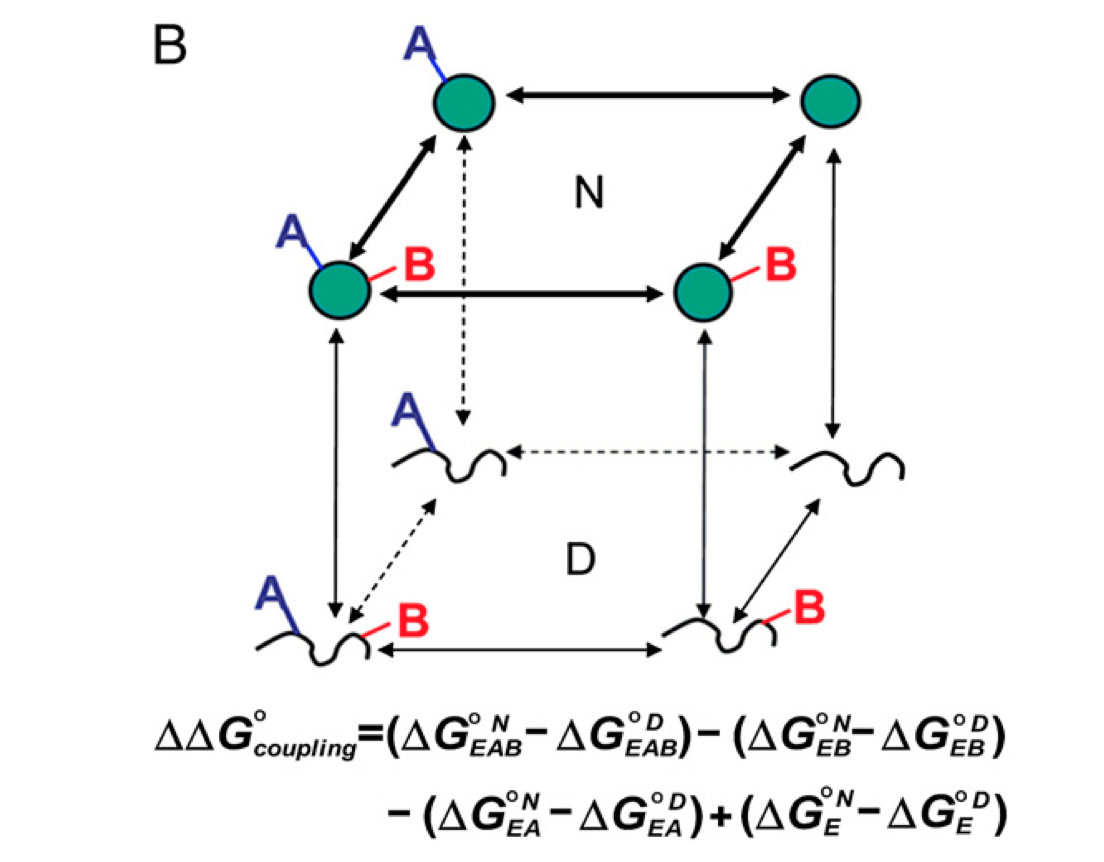
\includegraphics[width=8.6cm]{doubleMutant.png}
\caption{\label{f:DoubleMutant} { Taken from \cite{Cho2014} }}
\end{figure}

\warning{Where should this go?  There's nothing else to really add here, I just think it's nice that the cumulant framework gives an easy way to think about double mutant cycles.  This might make a nice paragraph in section II when we introduce the decomposition.  }


\section{Results}
\warning{Do we want to put anything here?  We could leave this as just a theory paper and leave out real results, or we could put in numerical results (like my CBR test script) or some real results (from old CCR calculations?).  I'm fairly against doing any new or complicated simulations}

\section{Conclusions}
 
 
\clearpage

\bibliographystyle{h-physrev}
\bibliography{Decompositions}

\end{document}


